\documentclass[11pt]{article}
\usepackage{amsmath, amssymb}
\usepackage{geometry}
\geometry{margin=1in}
\usepackage{fancyhdr}
\usepackage{lastpage}
\usepackage{parskip} % Better paragraph spacing
\usepackage{titlesec} % Better section formatting
\usepackage{graphicx}
\usepackage{float}
\usepackage[most]{tcolorbox}
\usepackage{lmodern} % Better font rendering


% Define commands for reusable content
\newcommand{\coursename}{COM-402 Information Security and Privacy}
\newcommand{\lecturenum}{02}
\newcommand{\lecturedate}{\today}

% Configure section spacing
\titlespacing*{\section}{0pt}{2ex plus 1ex minus .2ex}{1.5ex plus .2ex}
% Header / Footer
\pagestyle{fancy}
\fancyhf{}
\fancyhead[L]{\coursename}
\fancyhead[R]{Lecture \lecturenum}
\fancyfoot[L]{EPFL - Computer Science}
\fancyfoot[C]{Author: Jonathan Dutoit}
\fancyfoot[R]{Page \thepage\ of \pageref{LastPage}}

\begin{document}

\begin{center}
  {\large EPFL - Computer Science} \\[0.5em]
  {\Large \textbf{\coursename}} \\[0.5em]
  {\large Lecture \lecturenum\ --- \lecturedate} \\[0.5em]
  {\large Author: Jonathan Dutoit} \\
  {\large Professor: Mathias Payer} \\
\end{center}

\vspace{2cm}

\begin{center}
  {\LARGE \textbf{Crypto Basics}}
\end{center}

\vspace{1cm}	

\section*{Learning Goals}

\begin{itemize}
	\item Basic of symmetric crypto (stream ciphers, block ciphers, operation modes)
	\item Data integrity (hash functions, message authentication codes)
	\item Authenticated Encryption
	\item Public-key Cryptography (Digital signature, Diffie-Hellman key exchange)
	\item Public Key Infrastructure (PKI)
	\item Case study: TLS
\end{itemize}

\section*{Goals of Cryptography}

\begin{itemize}
	\item \textbf{Confidentiality}: Data is only accessible with the correct key
	\item \textbf{Integrity}: Any modification of data can be detected
	\item \textbf{Authentication}: The author of a message can be identified
	\item \textbf{Non Repudiation}: The author of a message cannot deny being the author
\end{itemize}

\section*{Examples of Cryptographic Schemes}

\begin{itemize}
	\item Caesar's
	\item Vigenere
	\item Elliptic-Curve Crypto
	\item RSA
	\item Enigma

	Used during the second World War, cryptography became a very important tool. Enigma is one of the prime example which was thought to be secure, multi-dimensional rotation used by the Germans, broken by the British and Americans and used to intercept and decipher the messages.
	Weakness: 
	\begin{itemize}
		\item Beginning was always the weather or "Hi Hitler" which made it susceptible to known plain text attacks. Allowed the team to test if they correctly decoded the message (quick sanitization)  
		\item An A would never be encoded to another A due to the mechanical property of the multi-dimensional rotation. 
	\end{itemize}
\end{itemize}


\section*{Brief Look into the Past}

\begin{itemize}
	\item -50 Caesar's Cipher (substitution)
	\item ...
	\item Kerckhoffs' principle
	\item 1970s Data Encryption Standard (DES)
	\item 1970s Diffie-Hellman public key crypto
	\item 1970s Rivest, Shamir, Adleman RSA
	\item 1985 Elliptic curve crypto (ECC)
	\item 1990s MD5, SHA-1 hash algorithms
	\item 2001 SHA-2
	\item 2001 Advanced Encryption Standard (AES)
	\item 2015 SHA-3
\end{itemize}

\section*{Brief Look at the Present/Future}

If quantum computers ever come to exist, they will break many crypto algorithms (mainly asymmetric). 

\textbf{Current research}: Post-quantum crypto: 

more complicated but plausibly unbreakable by quantum computers

\textbf{Follow up from professor's view}: likes the idea of quantum computers because they are extremely powerful, but will this ever materialize? Will we have strong enough quantum computer to do actually useful things? 

As a student mentioned, we already have a quantum computer that have a couple of cubits but they are extremely expensive and limited. 

Can we see a path were we can extend the number of cubits towards where we can do some actually useful computation such as breaking cryptography? 

\textbf{Personal opinion}: a bit sceptic about it. We'll see, but it's definitely an interesting playground for cybersecurity.

\section*{Naive Approach to Encryption}

Two parties agree on an algorithm (e.g., rot13) and keep it secret. Caesar's cipher was as simple shift of letters.

If you know that it is a shift, it only takes 26 trials to break it (i.e., susceptible to brute force) 

\begin{tcolorbox}[
  colback=yellow!15,     % background color
  colframe=black!50,    % border color
  boxrule=1pt,       % border thickness
  arc=3mm,             % rounded corners
  left=4mm, right=4mm, top=2mm, bottom=2mm % padding
]
\textbf{1883 - \textbf{Kerckhoffs's principle}} \\

\\

A cryptosystem should be secure even if everything about the system, except the key, is public knowledge. 
\end{tcolorbox}

\section*{One-Time Pad}

Key is a random string at least as long as the plaintext.

\begin{itemize}
	\item XOR operation to encrypt and decrypt
	\item $0 \oplus 0 = 0$, $0 \oplus 1 = 1$, $1 \oplus 0 = 1$, $1 \oplus 1 = 0$
\end{itemize}

Encryption: $c = m \oplus key$ 

Decryption: $m = c \oplus key$

One-time pad is \textbf{perfect} in theory.

Practical disadvantages:
\begin{itemize}
	\item Requires truly uniform random one-time pad values
	\item Key \textbf{must not} be used more than once. If you have multiple ciphertexts, you can combine them, either getting the key or the message.
	\item Key length depends on the message length
		\begin{itemize}
			\item e.g., it needs a 1TB key to encrypt a 1TB disk
		\end{itemize}
\end{itemize}

So, it's perfectly secure but impractical. For all of the crypto systems that we look at, we want to get as close to the one-time pad as possible, but being more practical. 

\section*{One-Time Pad Discussion}

Why use \textbf{XOR} and not \textbf{addition}?
\begin{itemize}
	\item I.e. ciphertext = plaintext + key
	\item \textcolor{red}{Potential information leaks! (violates confidentiality}. 
\end{itemize}

Ex: messages and keys chosen from the space of positive integers
\begin{itemize}
	\item Let plaintext = 3, key = 10
	\item Ciphertext = 3 + 10 = 13
	\item \textcolor{red}{Adversary can infer that plaintext < 13 !}
\end{itemize}


\section*{Symmetric Crypto}

Encryption and Decryption are done with the \textbf{same key} hence symmetric.

Solves the problem of transferring large amounts of confidential data

Reduces security to the problem of transferring a symmetric key (\textbf{key exchange})

% Quick centered image
\begin{figure}[H]
    \centering
    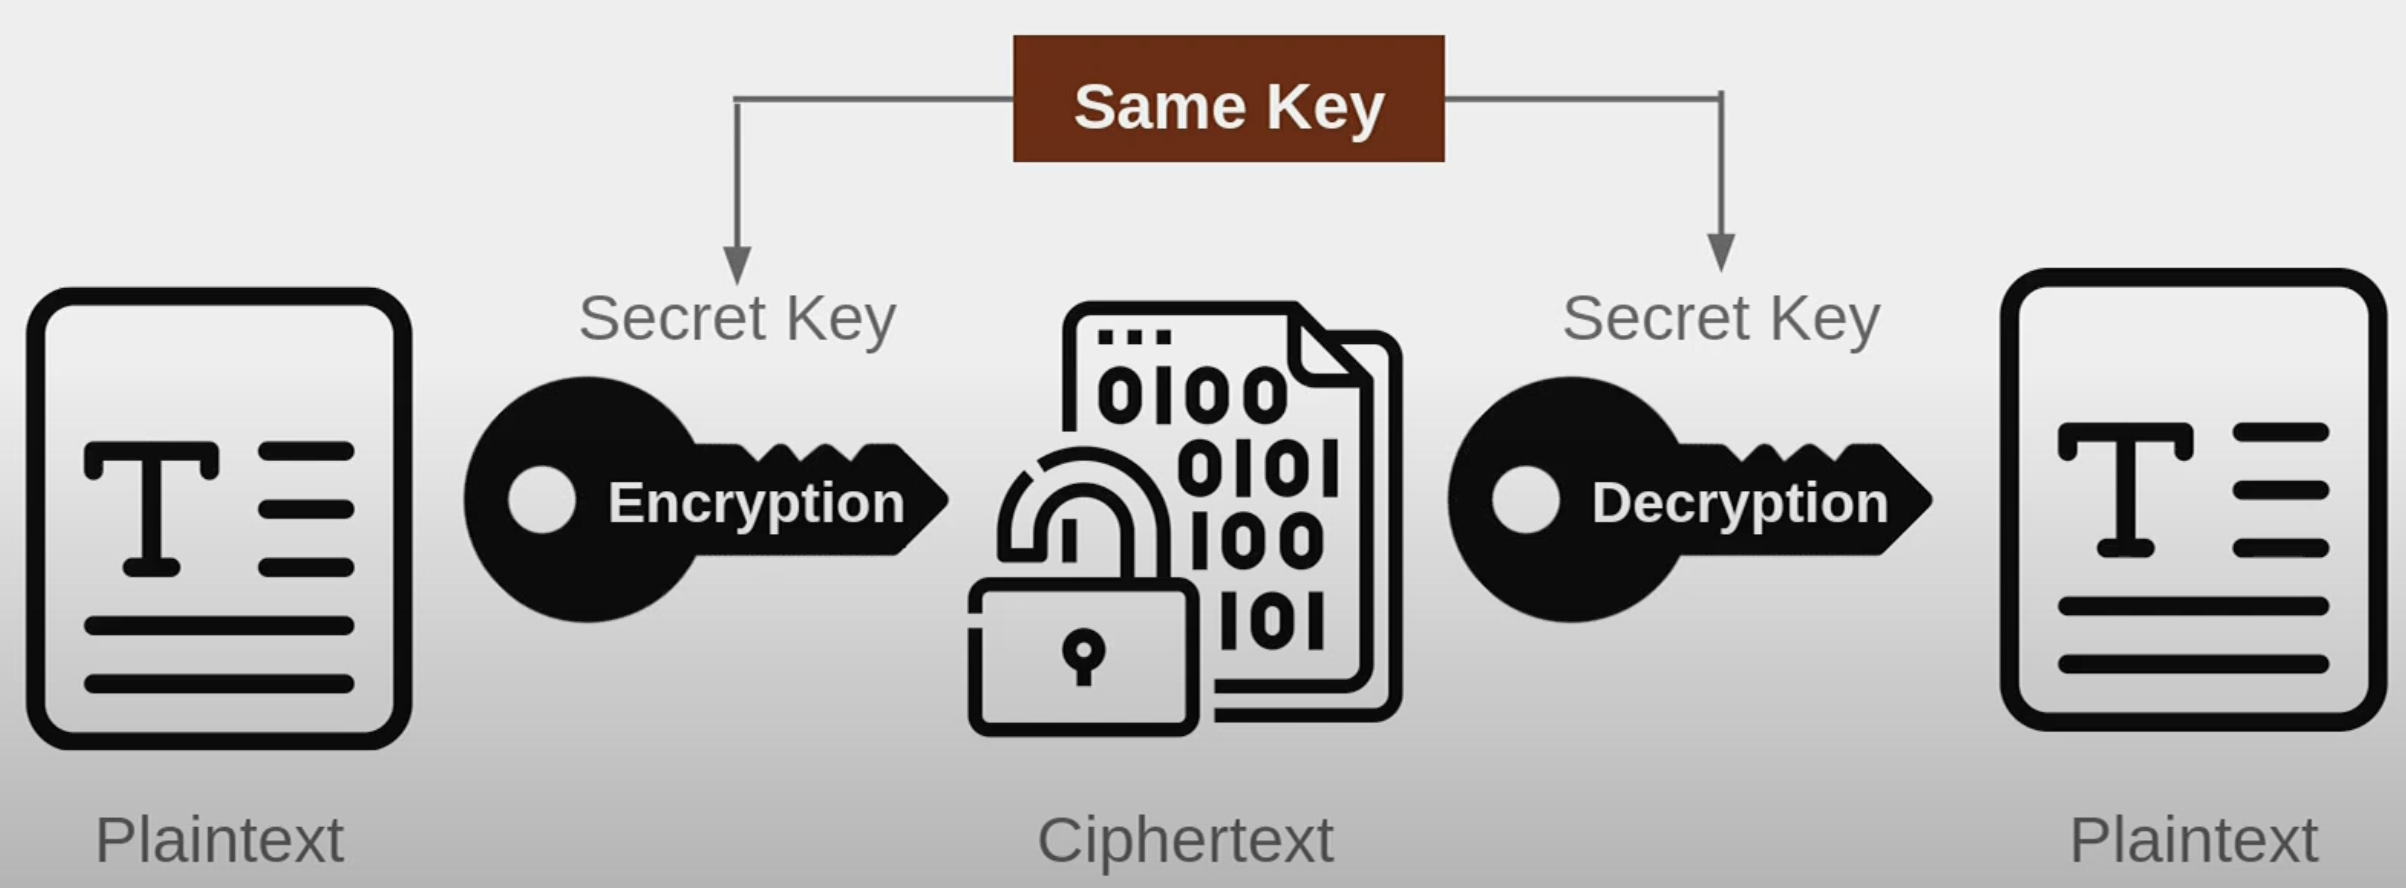
\includegraphics[width=1\textwidth]{symmetric-crypto}
    \label{fig:LABEL}
\end{figure}

\section*{Stream Cipher}

Use Pseudo Random Generator to expand a short seed into a stream of random bits

\[
	{\{0, 1\}}^{k} \Rightarrow {\{0, 1\}}^{n}, n > k
.\]

\begin{itemize}
	\item n-k bit stretch
	\item Use part of output as new seed
	\item Can encrypt data of arbitrary length
        \item Stream Cipher: XOR message and pseudorandom pad
	\item E.g., Salsa20, Chacha20
\end{itemize}

\section*{Limitation of Stream Ciphers}

Two possible pitfalls with stream ciphers:

\textbf{Malleability}: Flipping one bit of the ciphertext will flip the same bit in the plaintext
\begin{itemize}
	\item e.g., if you know which bit encodes the sign of a value you can change a payment of $100 to -$100
	\item you should always add an \textbf{integrity check} when encrypting data!
\end{itemize}

\textbf{Cipher reuse}: if two cleartexts are encrypted with the same cipher-stream, then: 

$M_1 \oplus M_2 = C_1 \oplus C_2$

\begin{itemize}
	\item If you know bits of one message, you can deduce the corresponding bits of the other message: $M_2[k] = M_1[k] \oplus C_1[k] \oplus C_2[k]$
	\item You should always use unique \textbf{seed} to create a pseudorandom cipher-stream
\end{itemize}

\section*{Block Cipher}

Encrypts \textbf{fixed size} blocks of data

\begin{itemize}
	\item a \textbf{padding scheme} is used to fill the last block
	\item a \textbf{mode of operation} to combine multiple blocks
\end{itemize}

Data Encryption Standard (\textbf{DES}):
\begin{itemize}
	\item block size 64 bits (too short, collisions)
	\item key size 56 bits (too short, can be brute forced)
\end{itemize}

\begin{tcolorbox}[
  colback=red!15,     % background color
  colframe=black!50,    % border color
  boxrule=1pt,       % border thickness
  arc=3mm,             % rounded corners
  left=4mm, right=4mm, top=2mm, bottom=2mm % padding
]

Don't use DES (or triple DES), both are deprecated
\end{tcolorbox}

Advanced Encryption Standard (\textbf{AES}):
\begin{itemize}
	\item block size 128 bits
	\item key size 128/192/256 bits
	\item hardware support (e.g., Intel, AMD, ARMv8)
\end{itemize}

\begin{tcolorbox}[
  colback=green!15,     % background color
  colframe=black!50,    % border color
  boxrule=1pt,       % border thickness
  arc=3mm,             % rounded corners
  left=4mm, right=4mm, top=2mm, bottom=2mm % padding
]
When in doubt, use AES
\end{tcolorbox}

\section*{Block Cipher: AES (Rijndael)}

\begin{minipage}{0.6\textwidth}
	\begin{itemize}
		\item A block cipher shuffles input on a per-block basis \\
		\item Each output byte depends on all input bytes \\
		\item Multiple rounds ensure thorough shuffling \\
	\end{itemize}
\end{minipage}
\hfill
\begin{minipage}{0.4\textwidth}
\centering
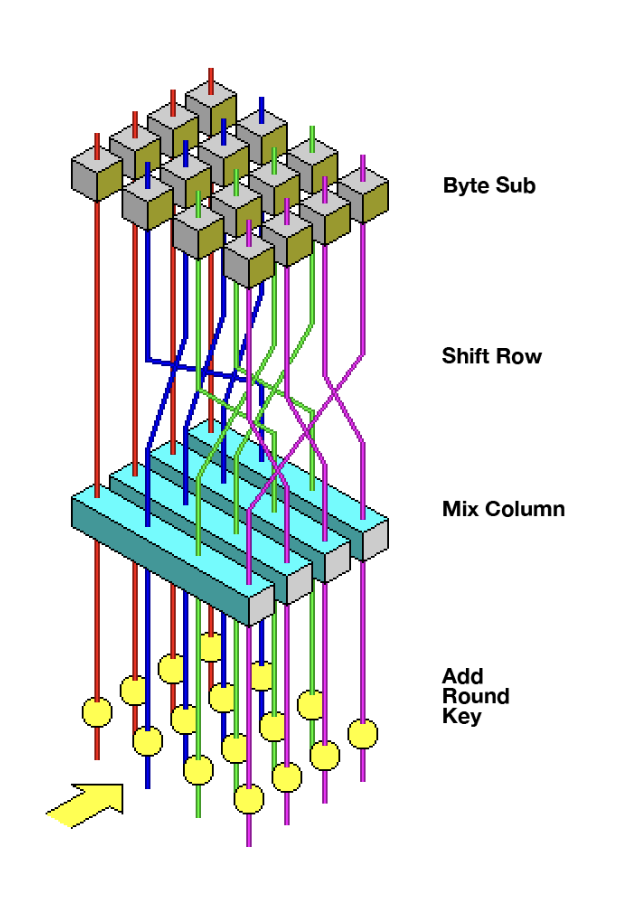
\includegraphics[width=\linewidth]{aes}
\end{minipage}


\section*{Modes of Operation: ECB}

\textbf{ECB}: Encrypt each block separately, with the same key

% Quick centered image
\begin{figure}[H]
    \centering
    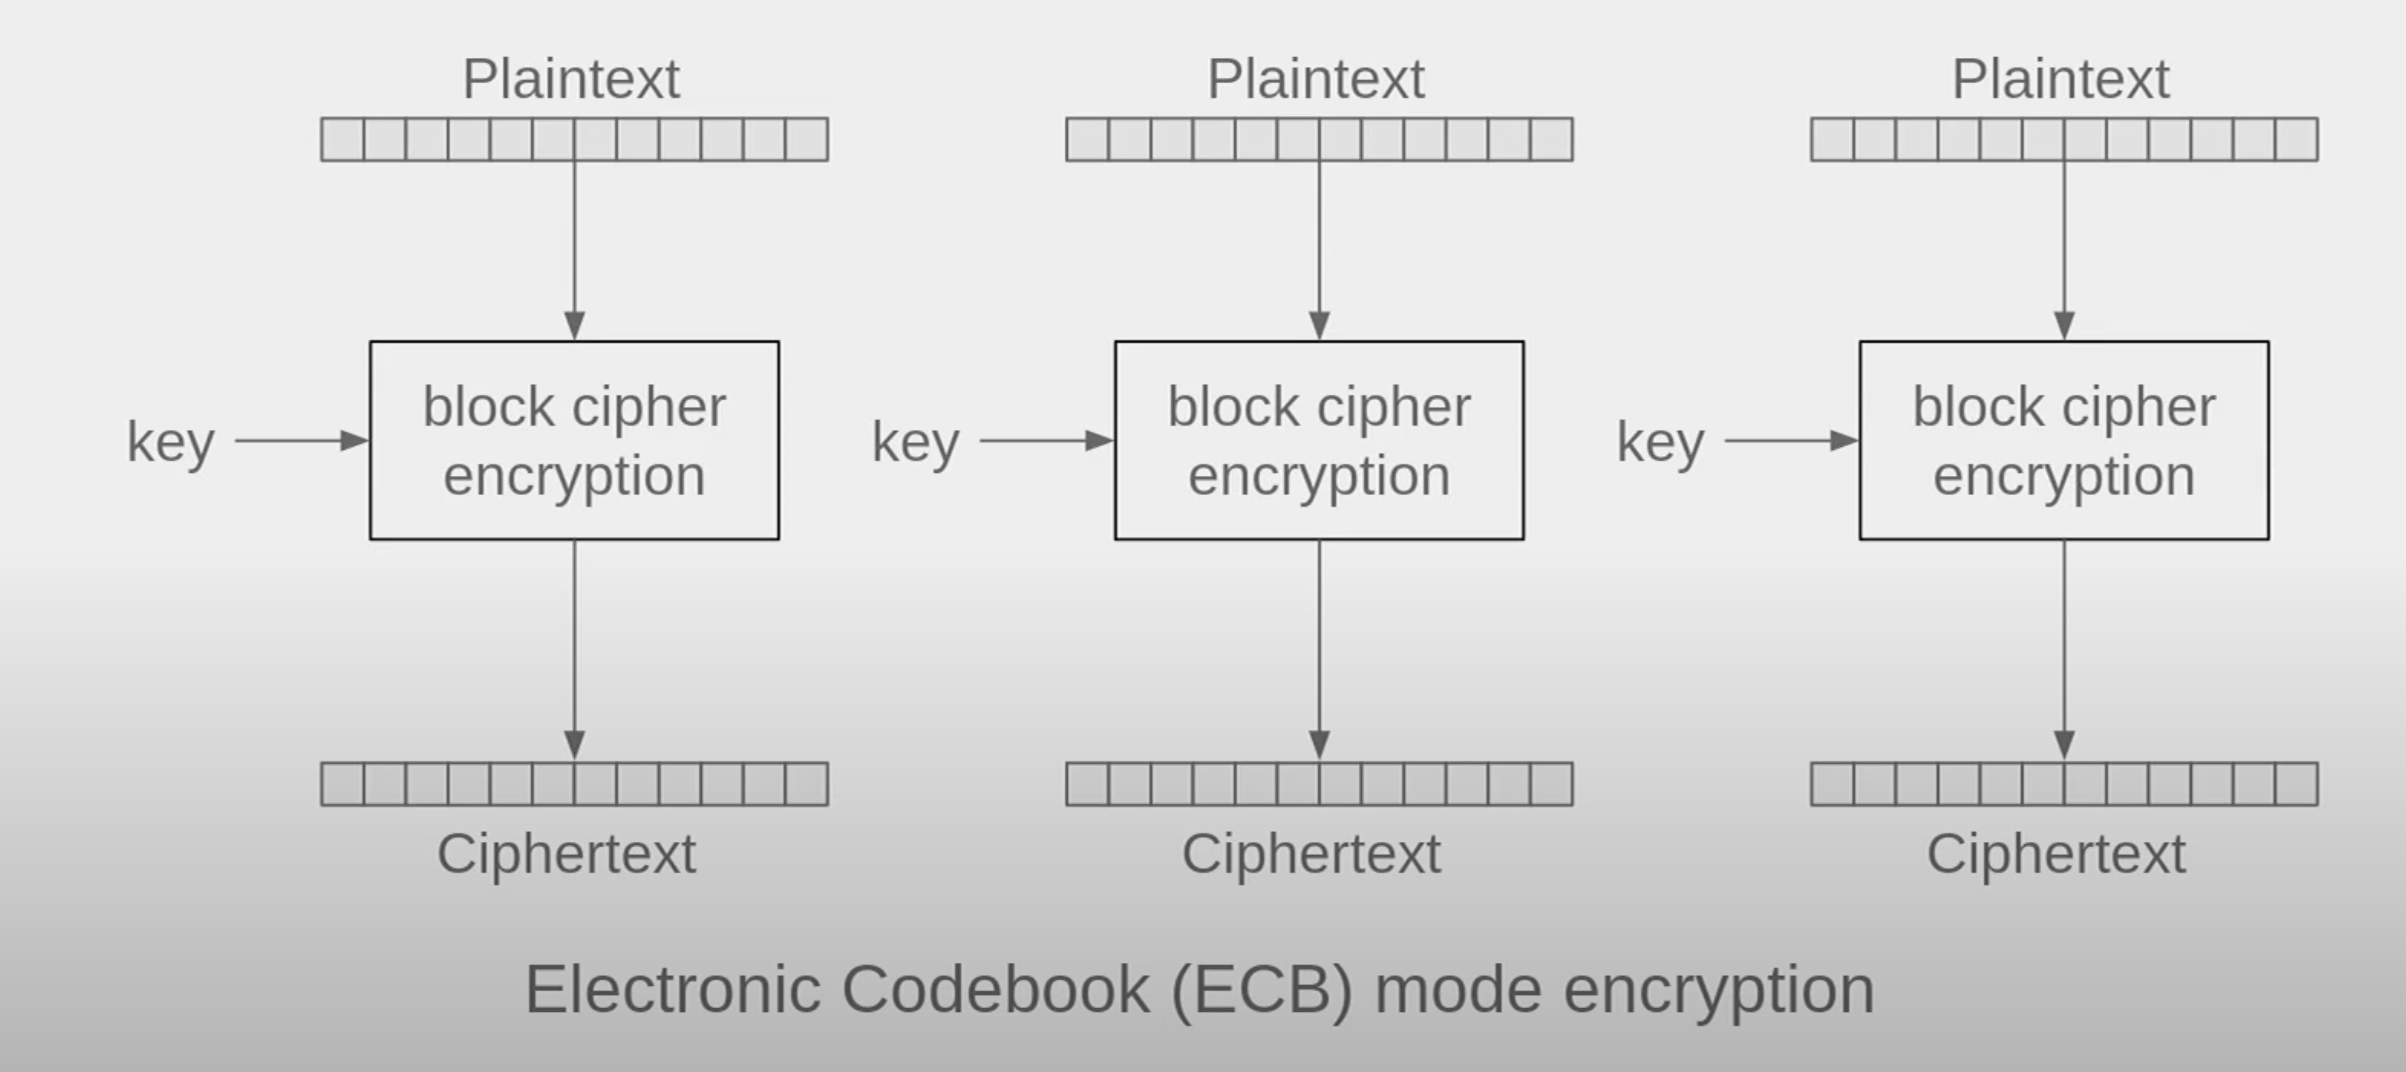
\includegraphics[width=0.7\textwidth]{ecb}
    \label{fig:LABEL}
\end{figure}

\textbf{Problem}: You can see patterns in the ciphertext. If you have a colored imaged, you can see the shape: 

% Quick centered image
\begin{figure}[H]
    \centering
    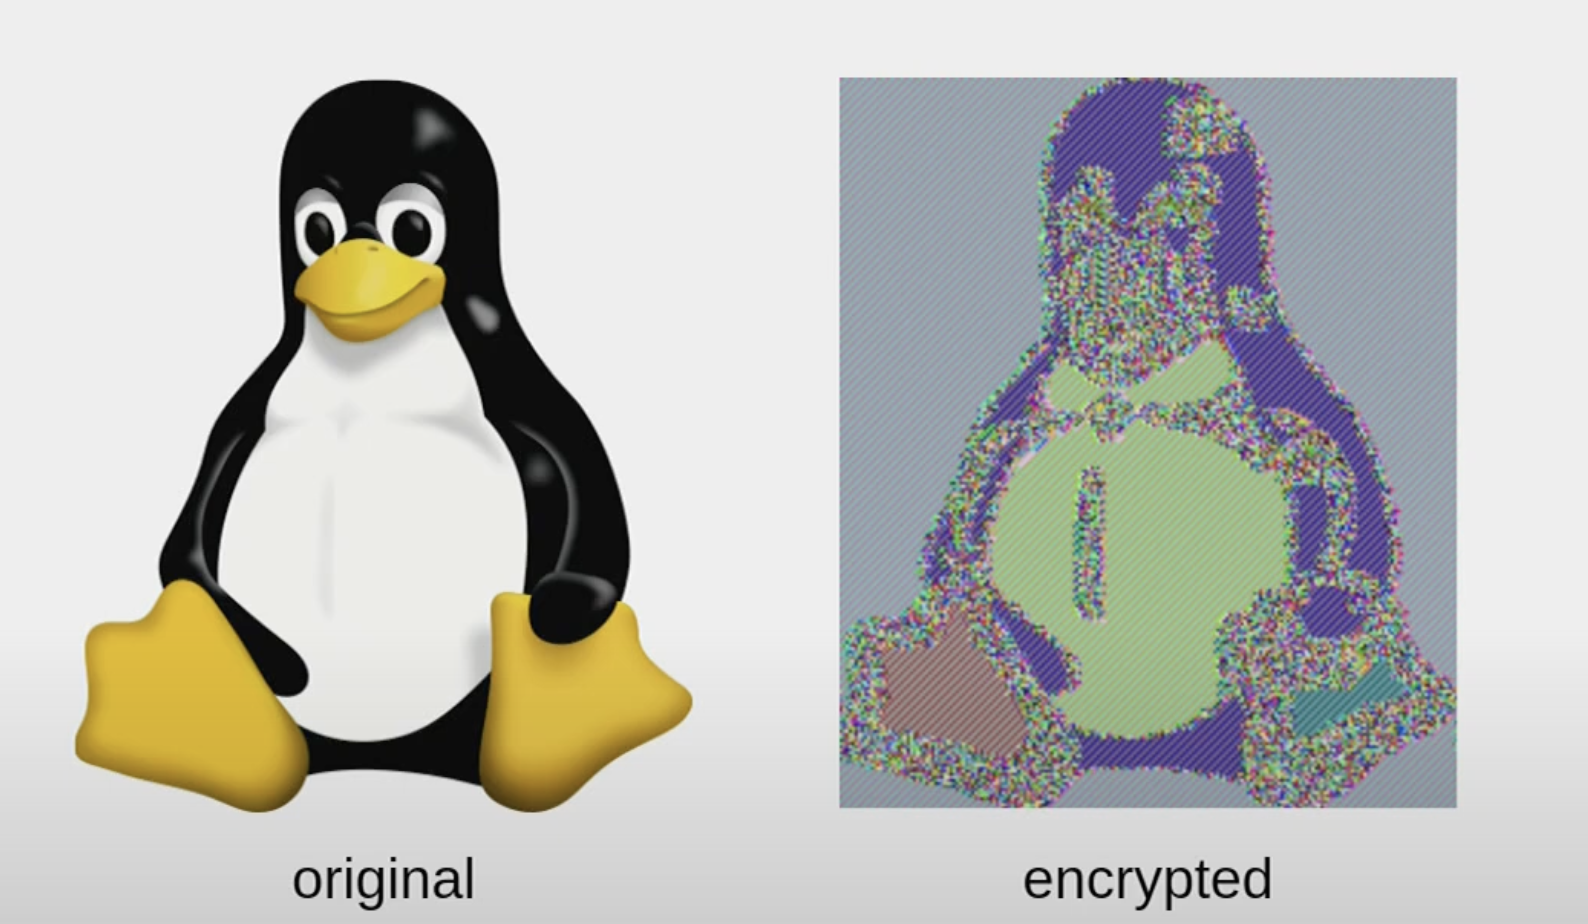
\includegraphics[width=0.7\textwidth]{penguin}
    \label{fig:LABEL}
\end{figure}



\section*{Modes of Operation: CBC}

Introduces the use of an Initialization Vector (IV) for the first block

% Quick centered image
\begin{figure}[H]
    \centering
    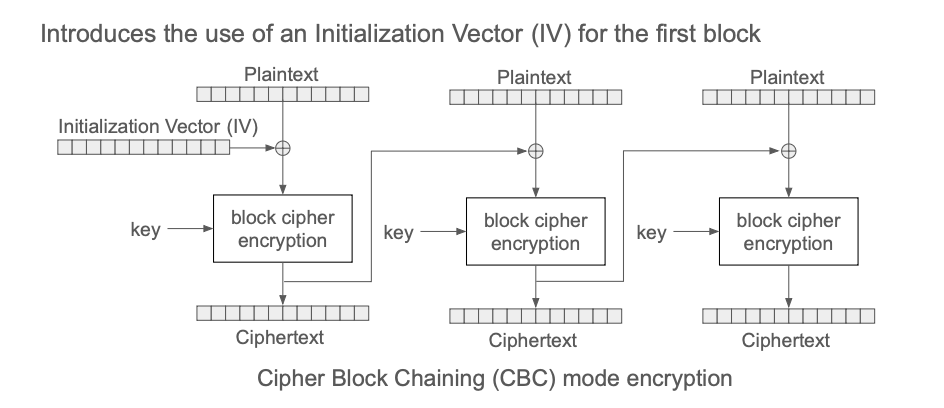
\includegraphics[width=0.7\textwidth]{cbc-encryption}
    \caption{Cipher Block Chaining (CBC) mode encryption}
    \label{fig:LABEL}
\end{figure}

Each ciphertext block acts as IV of the next block. 

Decryption is the opposite of encryption. 

% Quick centered image
\begin{figure}[H]
    \centering
    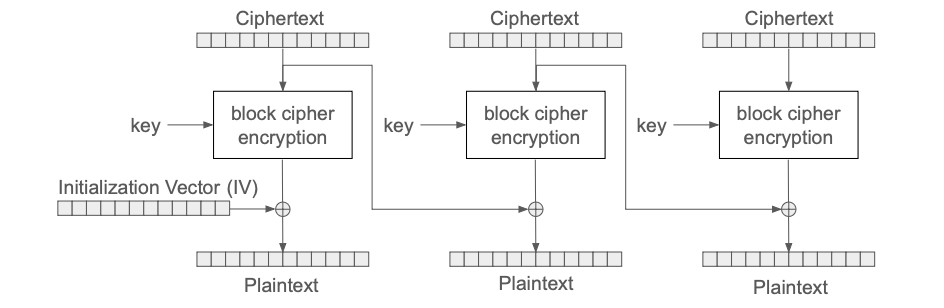
\includegraphics[width=0.7\textwidth]{cbc-decryption}
    \caption{Cipher Block Chaining (CBC) mode decryption}
    \label{fig:LABEL}
\end{figure}

\begin{tcolorbox}[
  colback=gray!15,     % background color
  colframe=black!50,    % border color
  boxrule=1pt,       % border thickness
  arc=3mm,             % rounded corners
  left=4mm, right=4mm, top=2mm, bottom=2mm % padding
]
\textbf{CBC encryption does not reveal any structure} \\

You can no longer see the penguin...

\end{tcolorbox}

\section*{Quiz!}

What happens to decryption if a bit is a flipped due to a transmission error? 

\begin{itemize}
	\item does the error propagate to all following blocks?
	\item does it only affect the current block?
	\item none of the above?
\end{itemize}

\textbf{Answer:} A whole block is garbled, one bit of the next block is inverted. 

Some possible pitfalls in using CBC: 

\textbf{Malleability}: 
\begin{itemize}
	\item Flipping one bit of the IV will flip the same bit in the plaintext
	\item Flipping one bit in a ciphertext block flips the same bit in the next plaintext block and mangles the current block
	\item \textbf{Always} add an \textbf{integrity check} when encrypting data!
\end{itemize}

\textbf{Padding oracle attacks}:
\begin{itemize}
	\item The last block must be padded to obtain the correct block size
	\item If not carefully implemented, validation of padding can lead to leakage of the plaintext (e.g., in TLS, see Serge Maude nay's BCC padding oracle attack)
\end{itemize}

\newpage

\begin{center}
  {\LARGE \textbf{Data Integrity}}
\end{center}

\vspace{1cm}

\section*{Data Integrity}

\textbf{Integrity}: protects against unauthorized modification

integrity \neq confidentiality

Remember the malleability of stream and block ciphers: \textbf{it's easy to flip bits of the cleartext}

We need a primitive that: 

\begin{itemize}
	\item detects any modification of the message
	\item cannot be forged (circumvented) by an attacker
\end{itemize}

\section*{(Cryptographic) Hash Functions}

Goal: Take an arbitrary length input, and generate fixed length output

Cryptographers say they map a 'preimage' to an 'image' 

\section*{Properties of Hash Functions}

\textbf{Preimage resistance}:

\begin{itemize}
	\item Given a hash h, it is difficult to find a message m for which h = hash(m)
	\item This implies that the function is a one-way function (and P != NP) 
	\item Very useful for password hashing
\end{itemize}

Prevented attack: given a password hash, an attacker cannot recover the \textbf{matching} password.

\textbf{Second preimage resistance}:

\begin{itemize}
	\item Given a message $m_1$, it is difficult to find a second message $m_2$ such that $hash(m_1) = hash(m_2)$
\end{itemize}

Prevented attack: hashes protect integrity of messages, thus, an attacker cannot forge a message with the same hash as an existing message.

\textbf{Collision resistance}

\begin{itemize}
	\item It is difficult to find any two messages $m_1, m_2$ such that $hash(m_1) = hash(m_2)$
\end{itemize}

Possible attack: hashes are used in signatures. An attacker could show one preimage and have signed by a third party. The signature would also be valid for the other preimage.


\section*{Quiz!}

What is the complexity of randomly finding a 2nd preimage in a random function that generates 160 bit outputs (e.g., SHA-1)?

What is the complexity of randomly finding a collision in SHA-1? 

NB: if the hash function has some weaknesses, the complexity might be lower. 

\textbf{Answer}: 

\begin{tcolorbox}[
  colback=green!15,     % background color
  colframe=black!50,    % border color
  boxrule=1pt,       % border thickness
  arc=3mm,             % rounded corners
  left=4mm, right=4mm, top=2mm, bottom=2mm % padding
]
Collisions in naively: $2^{60}$ operations

better: $2^{80}$ operations

Hashing $2^{80}$ random messages would produce one expected collision based on the birthday paradox.

\end{tcolorbox}

\begin{tcolorbox}[
  colback=red!15,     % background color
  colframe=black!50,    % border color
  boxrule=1pt,       % border thickness
  arc=3mm,             % rounded corners
  left=4mm, right=4mm, top=2mm, bottom=2mm % padding
]

In practice, it took $2^{63.1}$ operations to find a preimage. 
\end{tcolorbox}

\section*{Example of Hash Functions}

\textbf{MD5}: 128 bits, chosen prefix collisions are easy (\textcolor{red}{do not use})

\textbf{SHA-1}: 160 bits, broken, collisions are difficult but possible
(\textcolor{red}{avoid})

\textbf{SHA-2}: 224/256/384/512 bits, not broken, but related to SHA-1
(\textcolor{green}{use})

\textbf{SHA-3}: 224/256/384/512 bits, no weakness know(\textcolor{green}{prefer})

\textbf{BLAKE3}: 224/256/384/512 bits, no weakness know, faster, not standard (\textcolor{green}{fine})

\begin{tcolorbox}[
  colback=yellow!15,     % background color
  colframe=black!50,    % border color
  boxrule=1pt,       % border thickness
  arc=3mm,             % rounded corners
  left=4mm, right=4mm, top=2mm, bottom=2mm % padding
]
Key takeway: complex enough to be hard to brute force but reasonable to compute. Which means that even on today hardware, we need to able to computer. Even on embedded systems too.  

\end{tcolorbox}

\section*{Message Authentication Codes (MAC)}

Similar to a hash function, but involves a symmetric key

The same key is used to generate the MAC and to validate it

If they key is know only to the two parties of an exchange, a correct MAC proves:

\begin{itemize}
	\item that the messages was not created by a third party (\textbf{authentication})
	\item that the message has not been modified (\textbf{integrity})
\end{itemize}

Typically based on a hash function (e.g. HMAC SHA-2) or on block ciphers (e.g. CBC-MAC-AES)

\newpage

\begin{center}
  {\LARGE \textbf{Authenticated Encryption}}
\end{center}

\vspace{1cm}

\section*{Confidentiality and Integrity}

\begin{minipage}{0.4\textwidth}

\textbf{Always} require both confidentially \textbf{and} integrity. \\

But should we add confidentially first or integrity? \\

Different approaches:

\begin{itemize}
	\item encrypt then MAC (e.g., in IPSec, \textcolor{green}{use whenever possible})
	\item MAC then encrypt (e.g., in TLS)
	\item encrypt and MAC (e.g., in SSH)
\end{itemize}


\end{minipage}
\hfill
\begin{minipage}{0.6\textwidth}
\centering
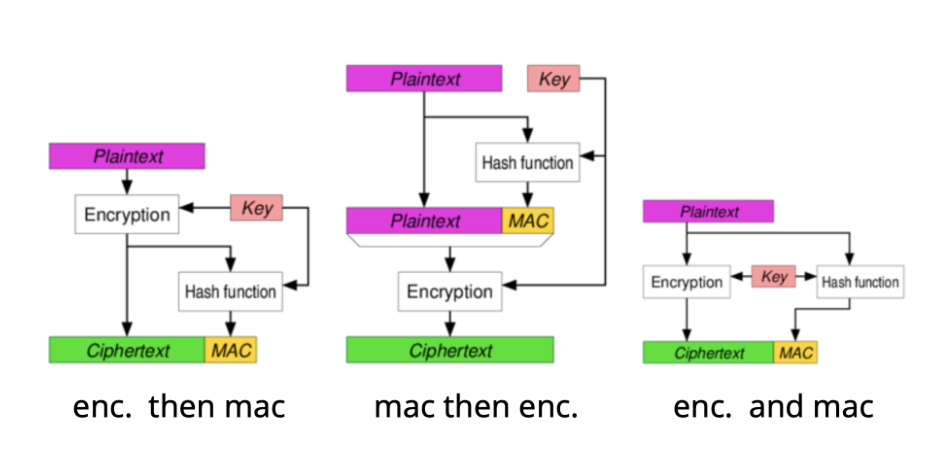
\includegraphics[width=\linewidth]{confidentiality-integrity}
\end{minipage}

\section*{Authenticated Encryption}

Modern encryption modes guarantee confidentiality and integrity

They include additional data that is authenticated but not encrypted: used for sequence numbers or other metadata 

\textbf{AEAD} (Authenticated Encryption with Associated Data)

Example: Galois/Counter Mode GCM

Idea: We're adding a counter that enumerates the different blocks and simply increments the counter that have been used and feed the counter in addition to the block cipher. 

% Quick centered image
\begin{figure}[H]
    \centering
    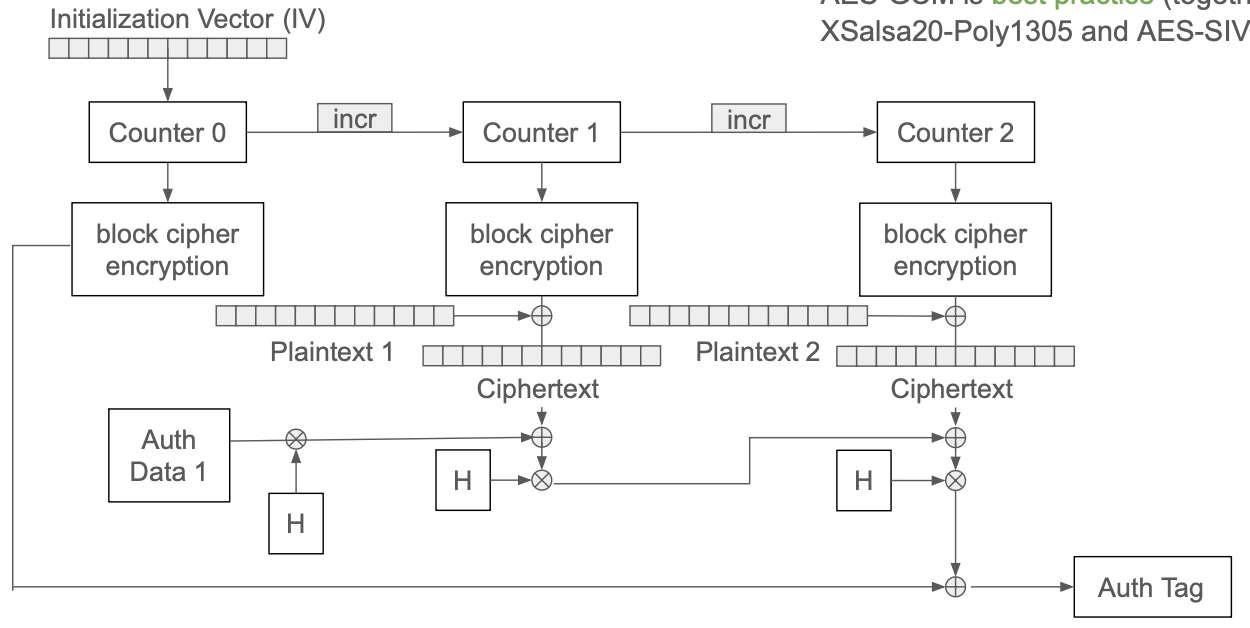
\includegraphics[width=1\textwidth]{galois}
    \label{fig:LABEL}
\end{figure}
Used with any block cipher, typically AES

AES-GCM is \textcolor{green}{best practice} (together with XSalsa20-Poly1305 and AES-SIV)

\vspace{0.5cm}

\begin{center}
  {\LARGE \textbf{Public-key Cryptography}}
\end{center}
Solves the problem of having to agree on a pre-shared symmetric key

Uses a \textbf{pair} of \textcolor{green}{public} and \textcolor{red}{private} key instead

Encryption with the \textcolor{green}{public} key guarantees that only someone with the \textcolor{red}{private} key can decrypt. 

Signing with the \textcolor{red}{private} key allows anyone with the \textcolor{green}{public} key to check validity.

The public key can be transferred \textbf{freely}, no need to keep it secret

Much better than symmetric keys!

\begin{tcolorbox}[
  colback=white!15,     % background color
  colframe=black!50,    % border color
  boxrule=1pt,       % border thickness
  arc=3mm,             % rounded corners
  left=4mm, right=4mm, top=2mm, bottom=2mm % padding
]
\textbf{Origin of Public-Key Crypto} \\

1975 Diffie and Hellman describe the idea of asymmetric crypto in "New directions in Cryptography".

\textbf{"...minimize the necessity of secure key distribution channels and supply the equivalent of a written signature...}
\end{tcolorbox}
\vspace{1cm}

\section*{Original Primitives}

Public and private key

\begin{itemize}
	\item Two keys: public is widely distributed, private is kept secret
	\item Must be hard to derive private from public
	\item May be easy to derive public from private
\end{itemize}

Operation: Encryption and decryption

\begin{itemize}
	\item Encrypt with public key, decrypt with private key
	\item Hard to decrypt without private key
\end{itemize}

Operation: Digital signature

\begin{itemize}
	\item Sign with private key, verify with public key
	\item Hard to create signature without private key
\end{itemize}

Interactive key exchange

\begin{itemize}
	\item Establish a shared secret key over an insecure communication channel
\end{itemize}

\section*{Digital Signatures}

Private key allows signer to generate an unforgeable signature that attests to the validity of message

Anybody can \textbf{verify} the signature using the public key

\textbf{Not} just encrypting with the secret key

Example signature schemes:
\begin{itemize}
	\item ECDSA and EdDSA (elliptic curve based, most common)
	\item BLS (pairing based, aggregatable, should be used more imo)
	\item DLithium (lattice-based), SPHINCS+ (hard-based). Post Quantum!
\end{itemize}

\textbf{Usage example}: software-update distribution

\begin{itemize}
	\item Your computer knows the public key of the software developer
	\begin{itemize}
		\item type apt-key list on Debian/Ubuntu to see them
	\end{itemize}
	\item Updates are signed
	\item Your computer can verify that the update indeed comes from the developer and that is has not been altered on its way
\end{itemize}

\textbf{Usage example}: authenticated email

\begin{itemize}
	\item If Alice knows Bob's public key, she can verify Bob's signature on messages
\end{itemize}

\textbf{Usage example}: Contacts
\begin{itemize}
	\item In Switzerland, you can sign contracts with digital signatures
\end{itemize}

\section*{Diffie-Hellman Key Exchange}

Alice and Bob want to exchange data securely. Suppose Eve can listen to any messages in our scenario. 

\textbf{Solution 1}: Alice and Bob agree on key ahead of time (this is the symmetric key from earlier). The difficulty comes from agreement of the key. How can we make this without having to agree on the key?

\textbf{Solution 2}: Multiple round-trips. Alice and Bob exchange multiple messages. Alice locks the box with her lock. Sends it over and Bob locks the box with his lock and sends it back. Alice removes her lock and etc...

\newpage

\textbf{Diffie-Helmman Key Exchange}

% Quick centered image
\begin{figure}[H]
    \centering
    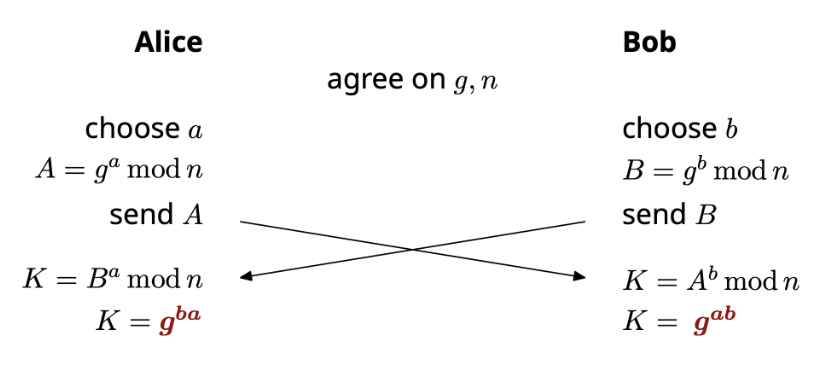
\includegraphics[width=0.7\textwidth]{diffie-hellman}
    \caption{By exchanging the public values A, B, and combining them with their private values b, a, Alice & Bob can create a shared secret K}
    \label{fig:LABEL}
\end{figure}

An attacker who observes A and B cannot find K

\textbf{Security Properties}

The reverse function of $A = g^{a} \% p$ is difficult (hard) due to discrete logarithm. Of course, numbers $p$ and  $g$ but be chosen well (large enough). Standard usually define  $p$ and  $g$

\textbf{Problem}: Powerful man in the middle attack. Mallory (malicious attacker) can do a Diffie-Hellman exchange with both Alice and Bob, thus having both keys to communicate with both of them. 

\begin{tcolorbox}[
  colback=red!15,     % background color
  colframe=black!50,    % border color
  boxrule=1pt,       % border thickness
  arc=3mm,             % rounded corners
  left=4mm, right=4mm, top=2mm, bottom=2mm % padding
]
Man in the middle may break Diffie-Hellman
\end{tcolorbox}

\begin{tcolorbox}[
  colback=green!15,     % background color
  colframe=black!50,    % border color
  boxrule=1pt,       % border thickness
  arc=3mm,             % rounded corners
  left=4mm, right=4mm, top=2mm, bottom=2mm % padding
]
Must authenticate each other using, e.g., public keys
\end{tcolorbox}

\section*{RSA Encryption}
Goals:

\begin{itemize}
	\item Alice wants to receive messages from any sender (\textcolor{blue}{confidentiality})
	\item Alice wants to prove message authorship to any receiver (\textcolor{blue}{integrity/authenticity})
\end{itemize}

Public key cryptography setup:
\begin{itemize}
	\item Alice generates $(sk, pk)$
	\item Alice distributes $pk$, keeps  $sk$ secret
\end{itemize}

RSA:
\begin{itemize}
	\item Pick primes p, q, computer \textbf{n = pq}
	\item Compute  $\phi(n) = (p-1)(q-1)$
	\item Pick \textbf{e} such that $1 < e < \phi(n)$ and  $gcd(\phi(n), e) = 1$
	\item In practice, use small prime  \textbf{e = $2^{16} + 1$}
	\item Find \textbf{d} such that $e \cdot d \equiv 1 \  mod \ \phi(n)$. In other words, \textbf{d} is the modular inverse of \textbf{e}, ($d \equiv e^{-1} \ mod \ \phi(n)$)
	\item Key-pair: \textbf{sk = (d, n), pk = (e, n)}
\end{itemize}

Encryption and decryption
\begin{itemize}
	\item $Enc_{pk}(m)$ = $m^{e}$ mod n
	\item $Dec_{sk}(c)$ = $c^{d}$ mod n
\end{itemize}

Signing and verification
\begin{itemize}
	\item $Sign_{sk}(m)$ =  $m^{d}$ mod n
	\item $Verify_{pk}(m, s)$ = (m ==  $s^{e}$ mod n)
\end{itemize}


% Quick centered image

 \begin{figure}[H]
     \centering
     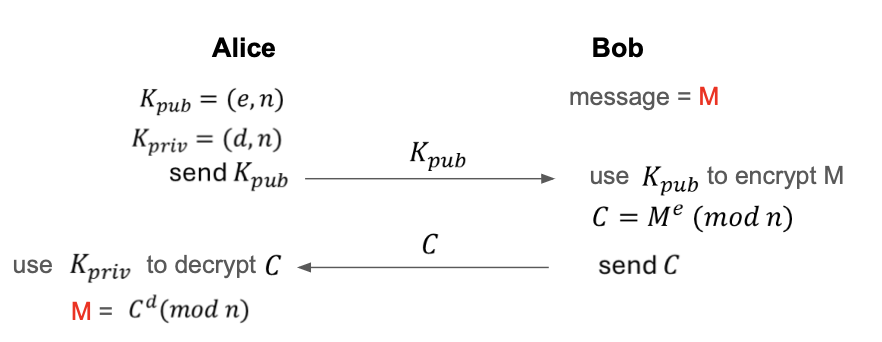
\includegraphics[width=0.7\textwidth]{rsa}
     \label{fig:LABEL}
 \end{figure}

But we usually want to sign large messages
\begin{itemize}
	\item RSA is expensive
	\item Solution: hash the message then sign the hash! \\
\end{itemize}


RSA can be broken by factoring $n$. Use a number of 3072 bits or more (for 128 bits of security)
Scheme above is trivially insecure. Use a padding scheme (preferably RSA-OAEP)


\section*{(Lab): Don't use textbook RSA}

\begin{itemize}
	\item Any \textbf{deterministic scheme} is not IND-CPA (Indistinguishably under chosen plaintext attack). This is the weakest notion of provable security that one would hope for in an encryption scheme, which is why in practice we are usually adding some randomized padding scheme on top of the textbook RSA. The attack works by simply outputting 0 if the \textbf{LoR(m, m)} to get an encryption of a message \textbf{m}. Then call \textbf{LoR(m, m')} with \textbf{m'} $\neq$  \textbf{m}, if the result is the same as the previous, return 0, else return 1. OR an simpler attack can work by observing that \textbf{0} to any power is \textbf{0} and \textbf{1} to any power is \textbf{1}.
	\item RSA is \textbf{malleable}. It satisfies multiplicative homomorphism: $(m_1m_2)^{e} \equiv m_1^{e}m_2^{e} \ mod \ n$. ($e$ is the public key) So even though you cannot call decrypt to the original ciphertext c, you can construct any new related ciphertext such as  $c' = c \cdot t^{e} \, mod \ n$ for some t, then call decrypt on c', then you can recover the plaintext for c by dividing this by t (modulo n). 
\end{itemize}


\section*{(Lab): Hastad's broadcast attack for RSA with low public explonent.}

\begin{tcolorbox}[
  colback=gray!15,     % background color
  colframe=black!50,    % border color
  boxrule=1pt,       % border thickness
  arc=3mm,             % rounded corners
  left=4mm, right=4mm, top=2mm, bottom=2mm % padding
]
\textbf{Chinese Remainder Theorem} \\

If the $n_i$ are pairwise coprime, and if $a_1, ..., a_k$ are any integers, then the system: \\

$ x \equiv a_1 \. (mod \ n_1)$ \\
$\ ... $ \\
$\ x \equiv a_k \. (mod \ n_k)$ \\

Has a solution, and any two solutions, say $x_1$ and $x_2$, are congruent modulo N, that is, $x_1 \equiv x_2 \ (mod \N)$.
\end{tcolorbox}

\begin{minipage}{0.6\textwidth}
If $N_1, N_2, N_3$ are relatively prime then by Chinese Remainder Theorem can combine \\

$C_1 = m^{3} \ mod \ N_1$ \\
$C_2 = m^{3} \ mod \ N_2$ \\
$C_3 = m^{3} \ mod \ N_3$ \\

To find $C = m^{3} \ mod \ N_1 \ N_2 \ N_3$. \\
Since $m^{3} < N_1 \ N_2 \ N_3$, thus $m \Leftarrow \sqrt[3]{C}$
\end{minipage}
\hfill
\begin{minipage}{0.4\textwidth}
\centering
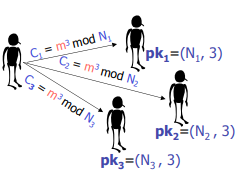
\includegraphics[width=\linewidth]{hastad}
\end{minipage}

\section*{Elliptic Curve Cryptography (ECC)}

Based on elliptic curves over finite fields

Used everywhere, e.g., can adapt Diffie-Hellman with different group operations

\textbf{Smaller} keys for \textbf{equivalent} security (e.g., 256 bit ECC comparable to 3072 bit RSA)

Popular curves offer fast performance:
\begin{itemize}
	\item curve25519
	\item Curve448
	\item NIST P256 (\textcolor{red}{controversial})
\end{itemize}

ECC is used for key exchange, e.g., in TLS: ECC Diffie-Hellman (ECDHE)

Used for signature: ECC Digital Signature Algorithm (ECDSA)

For example, Sony used ECDSA to sign the software of Playstation 3

\begin{itemize}
	\item ECDSA uses the private key for a nonce to gerate the signature
	\item The private key can be recovered if the same nonce is used in two signatures
	\item Easy to misuse, EdDSA improves on this (deterministic nonge generation)
\end{itemize}

Bitcoin addresses are a hash of an ECDSA public key

iMessages and iCloud keychan sync rely on ECDSA

\section*{Crypto Comparison}

Asymmetric is powerful but orders of magnitude slower than symmetric crypto

Asymmetric used to exchange a symmetric key, then symmetric key later.

All these algorithms are only safe with long enough keys (for 128 bits of security)

\begin{itemize}
	\item Symmetric: 128 to 256 bits
	\item Asymmetric: RSA 3072 bits, ECC 256 bits
	\item Hash functions: 256 bits
\end{itemize}

Cryptography is used in real life:

\begin{itemize}
	\item Symmetric: Kerberos
	\item Asymmetric: WPA3 (not possible to crack WiFi password), SRP
\end{itemize}


\newpage

\begin{center}
  {\LARGE \textbf{Public-key Infrastructure (PKI)}}
\end{center}

\vspace{1cm}

\section*{Key Distribution}

Cryptography reduces a security problem to one of key management

Public keys do not have to be secret, but still must be \textbf{authentic}

If a man in the middle can replace a public key, security guarantees are lost

We need a trusted third party to distribute the public keys

The Certification Authority (\textbf{CA}) certifies the keys by signing them. It does some validation before signing the keys

\begin{itemize}
	\item may ask for an email
	\item may ask for a copy of your passport
	\item this is documented in the Certificate Practice Statement (\textbf{CPS}) of the CA)
\end{itemize}

If we trust the key of the CA, we can trust all keys signed by the CA. A 'signed key' is a \textbf{certificate}. It contains at least:
\begin{itemize}
	\item the identity of the holder (subject)
	\item the validity date of the certificate
	\item the public key of the subject
	\item the signature by the CA
\end{itemize}

\textbf{Hierarchy of Trust}

Current browsers know a set of root CAs (144 root CAs in Firefox as of 11/2023). If there is a chain of signatures up to a trusted root, the browser trusts the certificate. 

\vspace{0.5cm}

\begin{center}
  {\LARGE \textbf{Case Study: TLS}}
\end{center}

\vspace{1cm}

\section*{TLS}

Transport Layer Security (TLS, previously know as SSL) provides confidentiality, integrity, and authentication

"The primary goal of TLS is to provide a secure channel between two communicating peers"

\textbf{Basic idea}: build your client-server app without security, add TLS, et voilà!

\section*{TLS Building Blocks}

The server is authenticated with a certificate. 

It proves its identity by signing some information received from the client with its private key. 

Client and server create a symmetric key using asymmetric crypto
\begin{itemize}
	\item EC Diffie Hellman \textbf{only} (since 1.3)
	\item Previously also supported standard Diffie-Hellman and key transfer
\end{itemize}

Once key established, used an AEAD to communicate (Authenticated Encryption with Associated Data)

\section*{TLS Cipher Suites (after 1.3)}

Algorithms to be used are specified in cipher suites: TLS\_AES\_128\_GCM\_SHA\_256

Key exchange and signatures default to ECDHE and RSA

Lesson from previous versions of the protocol:
\begin{itemize}
	\item Flexibility in cryptography can actually \textbf{hurt} security
	\item Better to stick to \textbf{same defaults}.
\end{itemize}

\begin{tcolorbox}[
  colback=red!15,     % background color
  colframe=black!50,    % border color
  boxrule=1pt,       % border thickness
  arc=3mm,             % rounded corners
  left=4mm, right=4mm, top=2mm, bottom=2mm % padding
]
Simplicity is key!
\end{tcolorbox}

\section*{TLS 1.3}
Removes old, no-longer-safe cipher suites, remove compression

Remaining cipher suites all use AEAD

Handshake
\begin{itemize}
	\item can be shorter in some cases
	\item is partially encrypted
\end{itemize}

Key exchange is always forward secure

Session resumption with pre-shared key (PSK)

About 63\% of website offer TLS 1.3 now

\section*{Perfect Forward Secrecy}

\textbf{Strong security notion}: session keys should not be compromised even if long-term secrets are.

Diffie-Hellman-like protocol offers Perfect Forward Secrecy (PFS)

At least since Ed. Snowden's revelations we know that:

\begin{itemize}
	\item Governments record a lot of traffic
	\item Governments exploit opportunities to steal private keys
\end{itemize}

\section*{TLS Handshake}

% Quick centered image
\begin{figure}[H]
    \centering
    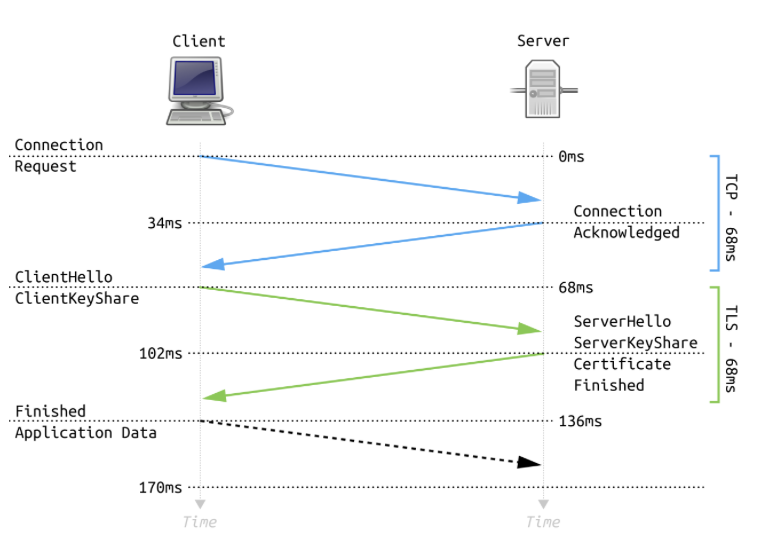
\includegraphics[width=1\textwidth]{tls-handshake}
    \label{fig:LABEL}
\end{figure}

\section*{TLS Uses Public and Symmetric Crypto}

Public key crypto:

\begin{itemize}
	\item The CA has signed the server's certificate (and its own root certificate)
	\item The server signs the key exchange to prove it hold the private key
	\item Elliptic curve Diffie Hellman is used to exchange a symmetric key
\end{itemize}

Symmetric crypto:

\begin{itemize}
	\item AES block cipher is used in CBC mode for encryption
	\item SHA has is used for HMAC, for key derivations
\end{itemize}

\section*{Implementing TLS}

Two major ways of implementing TLS

Use a new name and port (HTTPS, LDAPS, IMAPS, etc.):

\begin{itemize}
	\item HTTP on port 80  $\Rightarrow$ HTTPS on 443
	\item Start with a TLS handshake, security is mandatory
	\item Not compatible with clients that can't TLS
\end{itemize}

Use the STARTTLS command on the standard protocol
\begin{itemize}
	\item e.g., ESMTP (extended SMTP) on port 25
	\item client types STARTTLES if it want to start a handshake
	\item Opportunistic encryption, no guarantees
	\item MITM can pretend STARTTLS is not supported
\end{itemize}

\vspace{0.5cm}

\begin{center}
  {\LARGE \textbf{Deploying TLS on the Internet}}
\end{center}

\vspace{1cm}

\section*{Increasing Usage of TLS}

Using HTTPS everywhere would be better for Privacy and Security. This is quite recent, HTTP is being down-ranked and HTTPS is being preferred. 
\section*{Let's Encrypt: Free Certificates}

To able to create certificates that are trusted by all browser, you must undergo a costly certification

\begin{itemize}
	\item Prove that you protect your private keys
	\item Prove that you diligently validate the identity of your customers etc. 
\end{itemize}

The Internet Security Research Group (not for profit) found enough sponsors to certify a fully automated CA that gives certificates for free!

It's called \textbf{Let's Encrypt}

To obtain a certificate, you must place specific data
\begin{itemize}
	\item in a file on your web server, or
	\item in a DNS entry of your domain
\end{itemize}

Fully automatable: \textbf{no excuse for not using TLS!} 


\vspace{0.5cm}

\begin{center}
  {\LARGE \textbf{Attacks on HTTPS and Defenses}}
\end{center}

\vspace{1cm}

\section*{SSL Stripping and HSTS}

A MITM makes you believe that the site uses HTTP, not HTTPS

\begin{itemize}
	\item When you type a URL, your browser first connects using HTTP
	\begin{itemize}
		\item The server sends a redirect to HTTPS
		\item The MITM doesn't show you the redirect, your browser continues to use HTTP
	\end{itemize}
	\item Or, attacker replaces HTTPS with HTTP in the link of the pages that you visit
\end{itemize}

\section*{HSTS}
HTTP Strict Transport Security (HSTS) RFC 6797

The server sends an HTTP header indicating you must always use HTTPS.

\textbf{Strict-Transport-Security}: max-age=63072000; includeSubDomains;

Where '63072000' is one year.


\begin{tcolorbox}[
  colback=yellow!15,     % background color
  colframe=black!50,    % border color
  boxrule=1pt,       % border thickness
  arc=3mm,             % rounded corners
  left=4mm, right=4mm, top=2mm, bottom=2mm % padding
]
\textbf{Can you spot the weakness?} \\

If the MITM intercepts your very first connection to the site, they can hide the redirection to HTTPS

\begin{itemize}
	\item The client will \textbf{never see} the HSTS header
\end{itemize}

You can request that your domain be added to the HSTS-\textbf{preload} list \\

E.g., digitec.ch is on the list, your browser will never try HTTP when connecting to digitec
\end{tcolorbox}

\section*{Untrustworthy CAs}

A trusted CA (the root cert is in your browser) can give the MITM a trusted certificate in the name of \textbf{any} server

Using this, the server can intercept the traffic without you knowing.

Reasons for CA To hand out face certs:
\begin{itemize}
	\item The CA has been hacked (2021 Comodo was hacked, certificates were generate for, e.g., www.google.com, login.yahoo.com, login.skype.com)
	\item The CA is your company's CA. Companies often install their root certificate authorities so that they can MITM all your traffic for malware protection for it's employees 
	\item The government may have requested the certs in order to spy on its citizens (Syria, China, India, or France)
\end{itemize}

\section*{Protection Against Untrustworthy CAs}

\begin{itemize}
	\item \textbf{Certificate pinning}: client-side list of trusted certificates
	\begin{itemize}
		\item The developer of the client application stores the certificate of a trusted root CA, or intermediate CA in the client
		\item If the server show a certificate which is signed by this \textbf{pin}, it does not accept to connect, e.g., a mobile e-banking application only trusts certificates signed by an intermediate CA of the bank
	\end{itemize}
	\item \textbf{Certificate transparency}: public list of certificates
	\begin{itemize}
		\item Public signed logs of certs used in the internet. CAs submit all the certs they generate
		\item Servers can verify if the logs contain certs that they did not request. Then, somebody else requested a cert for their domain!
	\end{itemize}
\end{itemize}

\end{document}

